\subsection{Ej 1: TaskConsola}

\begin{algorithm}
 \caption{TaskConsola}
 \begin{algorithmic}[1]
 \Procedure{TaskConsola}{$n, bmin, bmax$}
   \State $srand(time(NULL))$ \Comment{seteo semilla de random}
   \For{$i\gets 0, n$}\Comment{n veces}
     \State{$random\_ number\gets modulo(rand(),\ bmax - bmin + 1) + bmin$}\Comment{[1]}
     \State{$Uso\_ IO(random\_ number)$}    
   \EndFor
 \EndProcedure
 \end{algorithmic}
\end{algorithm}

[1]: rand() retorna un número arbitrariamente grande.
Tomando su módulo en (bmax - bmin + 1) nos aseguramos que esté entre 0 y (bmax - bmin).\newline
Luego sumamos bmin, resultando un número entre bmin y bmax.

\subsection{Ej 2: Ejecutar TaskConsola con FCFS}

FCFS (First-Come First-Served) un scheduler simple en el cual los procesos son asignados al CPU en el orden en que estos lo requieren.\newline

\begin{wrapfigure}{l}{0.3\textwidth}
  \vspace{-30pt}
  \begin{center}
    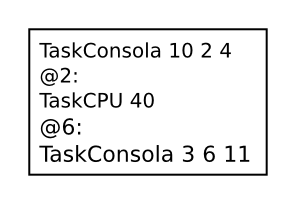
\includegraphics[width=0.25\textwidth]{./ej1y2/ej2_loteTareas.png}
  \end{center}
   \vspace{-30pt}
\end{wrapfigure}

Básicamente hay una sola cola (FIFO) de procesos 'Ready'. 
Cuando un proceso requiere CPU y éste está libre, se lo deja correr tanto tiempo como quiera y sin interrupciones.\newline

A continuación se muestran los gráficos para 1, 2 y 3 núcleos, usando SchedFCFS para el lote de tareas del cuadro.\newline

\vspace{10pt}
\textbf{1 Núcleo:}
\vspace{-20pt}
\begin{center}
 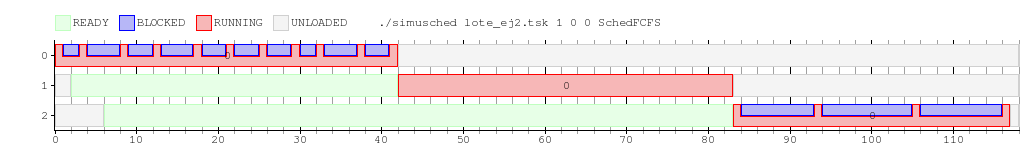
\includegraphics[scale=0.5]{./ej1y2/ej2_1core.png}
\end{center}

\vspace{10pt}

\textbf{2 Núcleos:}
\vspace{-20pt}
\begin{center}
 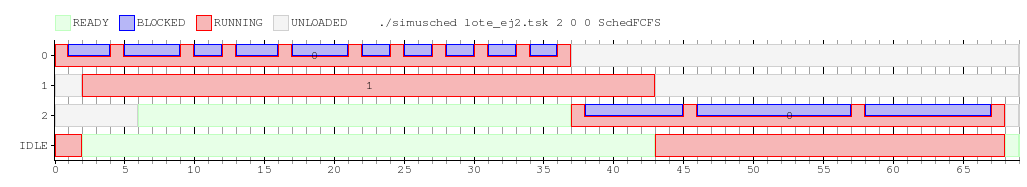
\includegraphics[scale=0.5]{./ej1y2/ej2_2core.png}
\end{center}

\vspace{10pt}

\textbf{3 Núcleos:}
\vspace{-20pt}
\begin{center}
 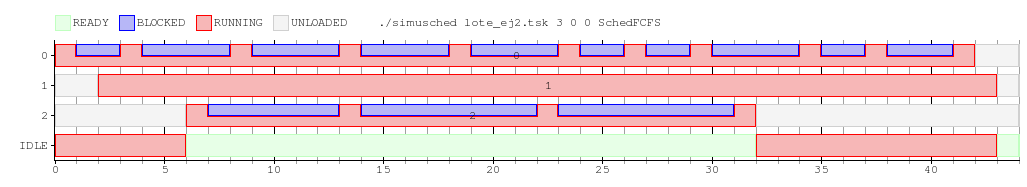
\includegraphics[scale=0.5]{./ej1y2/ej2_3core.png}
\end{center}


Obs: Los parámetros de costo de cambio de contexto y migración fueron seteados en 0 ya que en este scheduler en particular
no son tomados en cuenta. Porque núnca se desalojan las tareas ni se cambian de núcleo.

En los gráficos se hace evidente que a más cántidad de núcleos, mejor rendimiento, con FCFS.
Esto se debe a que FCFS no soporta múltitarea por sí sólo (ya que núnca desaloja a las tareas), sino que necesita varios núcleos para lograrlo.\newline

Las desventajas de FCFS son varias:

\begin{itemize}
\item Como ya dijimos, no soporta múltitarea.
\item Puede generar mucho 'waiting time'.\newline
	Si está ejecutando tareas muy largas las nuevas no entran hasta que éstas terminen.
\item No tiene buen rendimiento, a menos que se sepa la duración de las tareas de antemano.
\item Carece de 'fairness' i.e. no distribuye el/los procesador/es de forma justa entre las tareas.
\end{itemize}